\chapter{Indicadores de Desempenho da Manutenção}
\label{indicadores}

Os Indicadores de desempenho também conhecidos como KPIs, da sigla em inglês Key Performance Indicators, são métricas que quantificam a performance das organizações nas mais diversas áreas, de acordo com seus objetivos e metas. Eles são utilizados para monitorar os resultados da empresa e servem como referência para o processo de tomada de decisão e a criação de estratégias de melhoria. 

A manutenção, como a produtividade e a qualidade, por exemplo, possui diversos indicadores para sua gestão. Neste trabalho serão abordados os tradicionalmente usados, pois guardam uma correlação positiva com o desempenho e a segurança na empresa, todavia estes ao serem empregados devem ser individualizados para a função específica que se deseja controlar \cite{martorell1999}.

Qualquer que seja a forma que tomam os indicadores, os valores obtidos sobre eficiência, produtividade, segurança e disponibilidade, tem dois propósitos principais: decidir sobre o destino dos recursos e avaliar o desempenho do sistema depois que os recursos foram usados \cite{lofsten1998}. Assim, a ferramenta portadora dos indicadores permite identificar os desvios no desempenho dos equipamentos, e o controle que integra o laço de retro alimentação, que todo sistema de gestão bem implementado deve possuir. 

Segundo Martorell, \cite{martorell1999}, o primeiro passo para o desenvolvimento e implantação de KPIs deve ser a elaboração de um "panorama conceitual" para a avaliação da eficácia das tarefas que estão sendo executadas em qualquer setor de uma organização, seja ele a produção, o controle de estoque, os recursos humanos ou manutenção, por exemplo. O desenvolvimento desse panorama conceitual inicia-se com a coleta de informações básicas disponivéis nas fontes principais como o Sistema de Gerenciamento da Produção, Sistema de Informações da Manutenção e outras fontes importantes, se houver.

No caso da função Manutenção, Martorell forneceu orientações em um esquemático conceitual para a implementação do Sistema de Indicadores da Manutenção evidenciado na figura~\ref{Sistemas de Indicadores da Manutencao}, por meio da correlação dos objetivos da produção e os objetivos da manutenção.

\graphicspath{{figuras/}}
\begin{figure}[h]
\centering
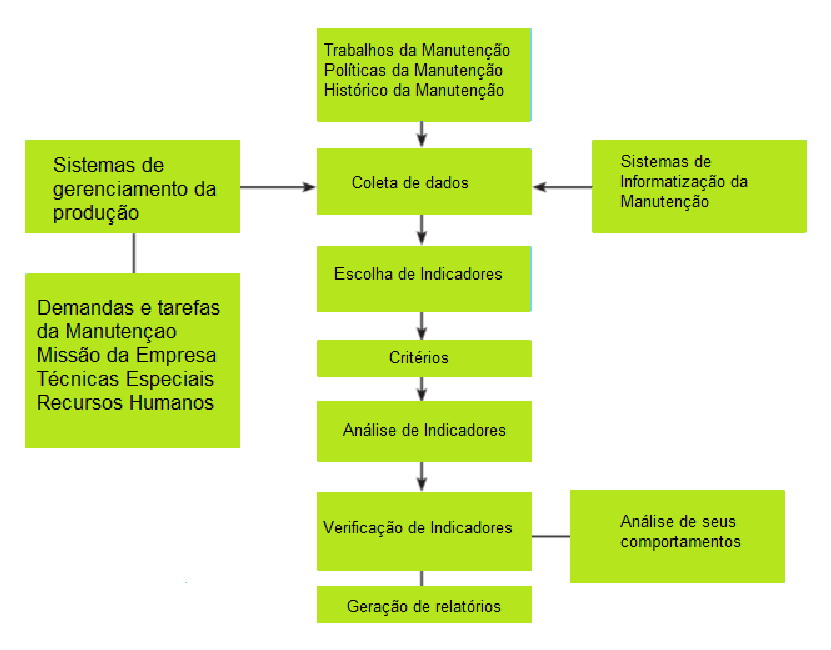
\includegraphics[width=0.8\textwidth]{Sistemas_de_Indicadores_da_Manuten_o.eps}
\caption{Sistemas de Indicadores da Função Manutenção.\textbf{Fonte: Autor. Adaptado de: Martorell at al:1996.}}
\label{Sistemas de Indicadores da Manutencao}
\end{figure}

O proxímo passo consiste na definição de Indicadores de desempenho, propriamente ditos, os quais estão intrínsecamente relacionados com os dados operacionais e incluem as fases de programação e execução das tarefas a serem desenvolvidas, e sua contribuição para o desempenho organizacional. No caso da função Manutenção, as informações operacionais são imprescindíveis para a implantação do Sistema de Indicadores de Manutenção devido sua natureza, que conforme \cite{martorell1999}, carecem ser utilizados em conjunto com as atividades operacionais, e com os processos usuais dos setores próprios da organização.

Deve-se ressaltar que nesta fase, também cabe a formulação de um panorama conceitual conforme ilustrou \cite{muchiri2011development} na figura~\ref{Desempenho da funcao manutencao}, o que facilita sua avaliação sob diferentes visões identificando elementos chaves e processos que dirigem a função manutenção para a entrega de resultados exigidos pelas metas de produção.
O panorama conceitual ilustrado resguarda a correlação das metas da função manutenção com a produção e os objetivos organizacionais e, assim, direciona os trabalhos da manutenção para a consecução dos objetivos de melhoria contínua dos equipamentos de produção e, consequentemente do sistema produtivo.

\graphicspath{{figuras/}}
\begin{figure}[h]
\centering
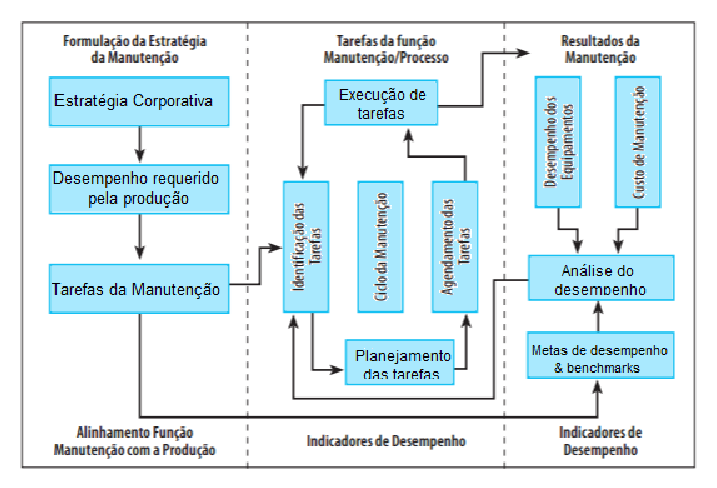
\includegraphics[width=0.8\textwidth]{desempenho_da_funcao_manutencao.eps}
\caption{Panorama conceitual para a análise da performance da função manutenção. \textbf{Fonte: Autor. Adaptado de Muchiri et al: 2011}}
\label{Desempenho da funcao manutencao}
\end{figure}

O panorama conceitual da Figura~\ref{Desempenho da funcao manutencao}, apresenta três partes fundamentais, a saber: O alinhamento da função manutenção com a produção, as tarefas da função manutenção/processos de manutenção e a análise dos resultados de desempenho, e revela que o controle de qualquer sistema depende da definição de indicadores de resultados apropriados, conforme o interesse do gestor. No entanto, os indicadores devem acompanhar o desempenho da manutenção nos seus processos principais e não em aspectos particulares, para permitirem uma visão geral da condição da manutenção.

A tabela~\ref{Indicadores de desempenho} mostra os principais indicadores e índices de desempenho normalmente utizados na avaliação da performance da função manutenção \cite{branco2006indicadores}.

\graphicspath{{figuras/}}	
\begin{table}[h]
\centering
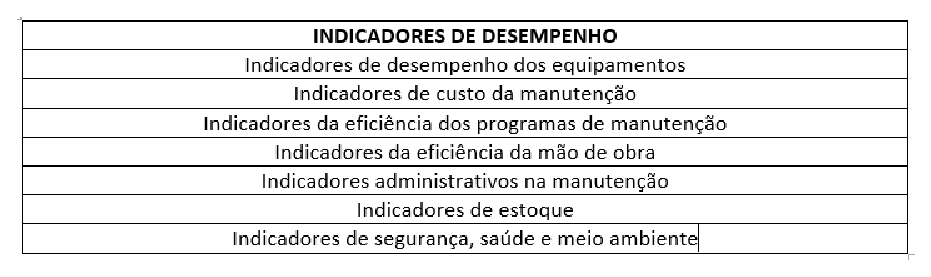
\includegraphics[width=0.8\textwidth]{IndicadoresBrancoFilho.eps}
\caption{Indicadores de Desempenho. \textbf{Fonte: Branco Filho: 2006}}
\label{Indicadores de desempenho}
\end{table}


Segundo Branco Filho \cite{branco2006indicadores}, somente os indicadores permitem uma quantificação e acompanhamento dos processos, eliminando a subjetividade e favorecendo as correções necessárias. Ou seja, os indicadores são dados chave para a tomada de decisão.

Sugere-se que os indicadores de desempenho, como os descritos na tabela~\ref{Indicadores de desempenho}, devem ser avaliados em blocos onde subconjuntos são analisados separadamente de acordo com seu significado. De modo que haja ao menos três subconjutos, separados em 1) Aqueles que monitoram o desempenho da manutenção nos níveis mais baixos, como os do ciclo de vida de um equipamento 2) Aqueles que impactam o sistema de execução das manutenções e 3) Aqueles que impactam a política global da manutenções na organização voltadas a segurança, ao custo e ao desempenho \cite{de2012indicadores}, conforme tabela~\ref{Niveis de indicadores de desempenho}.

\graphicspath{{figuras/}}
\begin{table}[h]
\centering
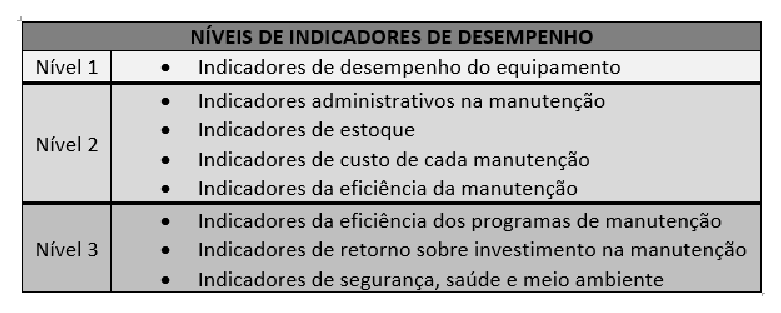
\includegraphics[width=0.8\textwidth]{niveisdeindicadores.eps}
\caption{Niveis de Indicadores de Desempenho. \textbf{Fonte: Autor}}
\label{Niveis de indicadores de desempenho}
\end{table}

Em relação ao nível 1, os principais indicadores de desempenho de um equipamento são:
\begin{itemize}
	\item TMF - Tempo Médio de Falhas ou Mean Time of Failures;
	\item TMEF - Tempo Médio entre Falhas ou Mean Time Between Failures;
	\item TMR - Tempo Médio entre Reparos ou Mean Time Between Repair;
	\item D - Fator Disponibilidade;
	\end{itemize}

Essas métricas medem atributos bem básicos do sistema. Duas dessas medidas são confiabilidade e disponibilidade. A definição convencional de confiabilidade \textbf{R(t)}, é a probabilidade de que o sistema esteja funcionando continuamente em um intervalo de tempo \textbf{[0,t]}.
Perto de confiabilidade está \textbf{Tempo Médio de Falhas (TMF)},  e \textbf{Tempo Médio Entre Falhas (TMEF)}. O primeiro é o tempo médio que o sistema opera até acontecer uma falha, enquanto o segundo é o tempo médio entre duas falhas consecutivas. A diferença entre as duas  é o tempo necessário para reparar o sistema depois da primeira falha. Estipulando \textbf{Tempo Médio de Reparo (TMR)}:

\begin{equation}
\label{eqn01}
	\mathbf{TMEF} = \mathbf{TMF} + \mathbf{TMR} 
\end{equation}

Disponibilidade, representado por \textbf{A(t)}, é a fração média de tempo sobre o intervalo \textbf{[0,t]} que o sistema está funcionando. Essa medida é apropriada para aplicações em que performance contínua não é vital mas onde seria caro ter o sistema fora por um período significativo de tempo. 
Disponibilidade pode ser interpretada como a probabilidade de que o sistema estará operante em um período de tempo aleatório, e só é significativo em sistemas que incluem reparo de componentes com defeito. Pode ser calculado por:

\begin{equation}
\label{eqn02}
	\mathbf{A} = \mathbf{\frac{TMF}{TMEF}} = \mathbf{\frac{TMF}{TMF + TMR}}
\end{equation}
Uma medida relacionada é Ap(t), que é a probabilidade do sistema operar em um determinado instante \textbf{t}.

É possível que um sistema de baixa confiabilidade tenha uma alta disponibilidade, por exemplo, um sistema que cai toda hora, mas se recupera em um segundo.

\section{Medidas Básicas de Tolerância a Falhas}
\label{falhas}

A análise das ferramentas de gestão e das técnicas de otimização da manutenção aumentam a disponibilidade dos equipamentos e instalações, na medida em que aplicam os conhecimentos da engenharia de manutenção \cite{xenos1998gerenciando}. Dentre as teorias comumente defendidas, temos a da "curva da banheira", que confronta em um gráfico bidimensional o tempo de uso versus a taxa de falhas dos equipamentos, conforme mostra a figura~\ref{Curva da banheira}.

\graphicspath{{figuras/}}
\begin{figure}[h]
\centering
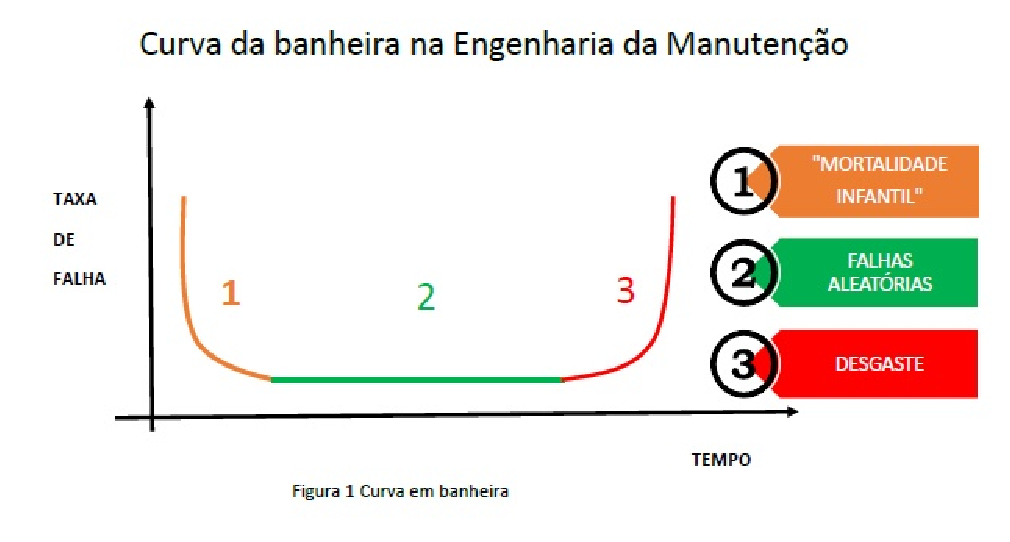
\includegraphics[width=0.8\textwidth]{curva_da_banheira.eps}
\caption{Teoria da curva da banheira \textbf{Fonte:A Curva da Banheira na Engenharia da Manutenção:2016.}}
\label{Curva da banheira}
\end{figure}

Conforme observado no gráfico acima, as frequências de ocorrência das falhas em um equipamento podem ser classificadas em 1) decrescente; 2) constante ou aleatória e 3) crescente, estando associadas ao estágio do ciclo de vida do equipamento.

\begin{itemize}
	\item \textbf{1) Decrescente:} Nesta fase, também denominada de "mortalidade infantil", ocorrem falhas advindas dos defeitos de projeto, de fabricação e de instalação. É caracterizada por uma alta taxa de falha no início de sua operação;
	\item \textbf{2) Constante ou aleatória:} Esta fase costuma ser denominada de vida normal ou fase de estabilidade do equipamento, uma vez que a taxa de falhas é aproximadamente constante e ocorrem aleatoriamente, estando associadas a aplicação de esforços acidentais e/ou erros de manutenção. A taxa de falha é menor do que nas demais fases;
	\item \textbf{3) Crescente:} Esta fase reflete o período de instabilidade próprio do fim da vida útil do equipamento, ou seja, o sistema e seus componentes apresentam falhas por desgaste natural, decorrente do seu uso. Há um aumento considerável da taxa de falha nesta fase.  
\end{itemize} 

O conhecimento da "curva da banheira" por parte das instituições auxilia no controle da manutenção, na determinação da vida útil, no estabelecimento do tempo de garantia e na adoção de medidas indispensáveis para o aumento da disponibilidade e confiabilidade dos equipamentos.

Koren e Krishna \cite{koren2007} dizem em seu livro \emph{Fault-Tolerant System} que todo tipo de tolerância a falhas é um exercício de explorar e gerenciar redundância. Redundância é a propriedade de ter mais de um recurso do que o minimamente necessário para o trabalho sendo feito. Quando acontece uma falha, a redundância é explorada par mascarar ou contornar essas falhas, mantendo o nível desejado de funcionalidade. Eles trazem quatro tipos de redundância: de hardware, de software, de informação e de tempo. Abaixo será relatado como os autores tratam os conceitos relacionados a \textbf{tolerância a falhas}. 

A tolerância a falhas tem como objetivo tornar máquinas mais confiáveis, por isso ela tem medidas próprias. Medida é uma abstração matemática, que expressa uma observação da performance de um objeto. O truque em definir medidas adequadas é manter o subsistema largo o suficiente para que o comportamento de interesse do usuário seja capturado, e ainda assim não tão largo, para que a medida não perca o foco. 

\section{Modelagem da falha de equipamentos eletrônicos}

Embora a maioria das causas que levam os equipamentos ao desgaste estejam ligadas a seu uso, eventualmente, podem ter ocorrido problemas durante o seu processo de fabricação, ocasionando a produção de componentes fora da especificação e mais frágeis. Estes equipamentos quais provavelmente irão apresentar problemas prematuros, quando colocados em operação. De acordo com Sanches (2010, p. 19) os equipamentos que apresentam defeitos/falhas provenientes dos processos de fabricação apresentam problemas em um período inicial, que em média corresponde a 5\% da sua vida útil – período conhecido como falhas prematuras ou precoces.

Ou quando se deseja melhorar as suas condições de uso, algumas delas estão relacionadas à escolha do equipamento mais indicado, ou quais modificações serão necessárias a serem feitas na infra-estrutura para adequadamente utilizá-lo.

Restabelecer características construtivas originais dos equipamentos, garantindo a eles um nível de desempenho esperado através da manutenção. 
Estas ações de correição e prevenção quando adotadas aumentam a eficiência operacional e o tempo de vida útil dos ativos da organização.

